\subsection{Arbres BSP en deux dimensions}
\subsubsection*{Définitions et notations}
L'arbre BSP (binary space partition) est la structure principale
intervenant dans l'algorithme du peintre. En deux dimensions, il est
utilisé pour stocker des ensembles de segments destinés à être affichés.


Soit
\begin{equation} \label{lin:forme}
f: \mathbb R^2 \to \mathbb R: (x, y)\mapsto ax +by
\end{equation}
une forme linéaire sur $\mathbb R^2$ non nulle, et $c\in\mathbb R$ un réel. Alors, il est possible de
partionner le plan $\mathbb R^2$ en trois sous-ensembles en le séparant
par la droite $D = \{v\in\mathbb R^n\mid f(v) = c\}$;
la droite $D$ elle-même et les demi-plans
$\{v\in\mathbb R^2\mid f(v) > c\}$ et
$\{v\in\mathbb R^2\mid f(v) < c\}$, notés respectivement $D^+$ et $D^-$
dorénavant
(voir figure \ref{sep:ill}). Ce choix de notation est lié à l'équivalence
$f(x)> c$ si et seulement si $f(x)-c>0$; $D^+$ est appelé
le demi-plan positif. De manière analogue, $D^-$ est
appelé le demi-plan négatif.


\begin{figure}[!h]
  \begin{center}
    \caption{Partition du plan par une droite et deux demi-plans}%
    \label{sep:ill}
    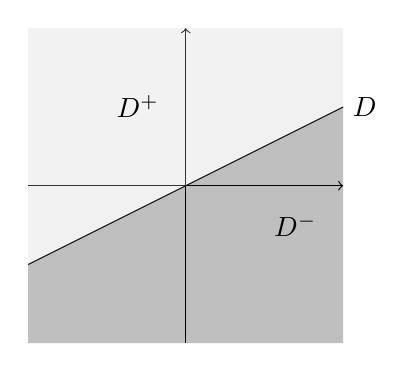
\begin{tikzpicture}
      \draw [->] (0, -2) -- (0, 2);
      \draw [->] (-2, 0) -- (2, 0);
      \draw (-2, -1) -- (2, 1) node[right] {$D$};
      \fill [black, nearly transparent] %
      (-2, -1) -- (2, 1) -- (2, -2) -- (-2, -2) -- cycle;
      \draw (1, -0.5) node[right] {$D^-$};
      \fill [black!20, nearly transparent] %
      (-2, -1) -- (2, 1) -- (2, 2) -- (-2, 2) -- cycle;
      \draw (-1, 1) node[right] {$D^+$};
    \end{tikzpicture}
\end{center}
\end{figure}

%%% Local Variables:
%%% mode: latex
%%% TeX-master: "../rapportGp1"
%%% End:


\begin{df}\label{def:bsp}
  Un arbre BSP $T$ est un arbre binaire tel que:
  \begin{enumerate}
  \item Chaque noeud contient un ensemble $S$ de segments (éventuellement
    vide).
  \item Chaque noeud contient une équation de droite $D\equiv f(x, y) = c$
    (où $f$ est une forme linéaire et $c$ est un nombre réel).
  \item Tout segment dans $S$ est contenu dans la droite $D$.
  \item Chaque segment stocké dans le fils gauche $T^-$ (resp.
    le fils droit $T^+$) d'un noeud est contenu dans le demi-plan
    $D^-$ (resp. $D^+$).
  \end{enumerate}
\end{df}
Les notations adoptées dans la définition \ref{def:bsp} seront employées
dans la suite de cette section.

\subsubsection*{Raisonnement mathématique: construction de l'arbre}
Afin de construire des arbres BSP à partir d'une liste $L$ de segments
du plan, il faut à chaque fois sélectionner une droite par laquelle
séparer l'espace.
Dans ce travail, seules les droites comportant un segment de $L$ sont
sélectionnées comme droites séparatrices. Cela permet notamment d'assurer
l'arrêt de l'algorithme de construction.

Le lemme suivant montre qu'il est possible d'obtenir une équation de droite
à partir d'un segment non dégénéré, en temps constant.

\begin{lem}\label{lem:droite}
  Soient $p_1 = (x_1, y_1)$ et $p_2 = (x_2, y_2)$ deux points distincts du
  plan. Une équation cartésienne de la droite  passant par $p_1$ et $p_2$
  est donnée par
  \begin{equation}
    \left(y_2 - y_1\right) x + \left(x_1 - x_2\right) y =
    \left(y_2 - y_1\right) x_1 + \left(x_1 - x_2\right) y_1
  \end{equation}
\end{lem}
\begin{proof}
  Le vecteur $(x_2 - x_1, y_2 - y_1)$ est un vecteur directeur de la droite.
  Alors $(y_2 - y_1, x_1 - x_2)$ est un vecteur normal de la droite ce qui
  implique que
  $$\left(y_2 - y_1\right) x + \left(x_1 - x_2\right) y = c$$ est une équation
  de la droite, où $c$ est à déterminer.
  Puisque le point $(x_1, y_1)$ appartient à la droite il suffit de poser
  $c = \left(y_2 - y_1\right) x_1 + \left(x_1 - x_2\right) y_1$
\end{proof}

Le lemme \ref{lem:droite} fournit une équation de la droite passant par
par deux points distincts en temps constant: il suffit d'effectuer
quelques opérations arithmétiques élémentaires pour déterminer les
coefficients intervenant dans l'équation.

Le choix du segment
pour la partition est effectué selon une heuristique (se référer à la section
\ref{heur:section}).
Une fois la droite $D$ choisie, l'arbre est construit récursivement.
Deux nouvelles listes, $L_d$ et $L_g$ sont créées pour construire récursivement
les sous-arbres gauche et droit.

Si un segment $s$ de $L$ est compris dans la droite $D$, il est stocké à
la racine de l'arbre, dans l'ensemble $S$. Si un segment est contenu dans
le demi-plan $D^+$ (resp. $D^-$), il est stocké dans la liste $L_d$ (resp.
$L_g$). Si seule une des extrémités se trouve sur la droite, le segment
est considéré commme appartenant au
 demi-plan auquel le reste du segment appartient.

Si une extrémité est dans $D^+$ et l'autre dans $D^-$, il est nécessaire
de briser le segment en deux parties, qui seront ensuite ajoutées à une des
listes selon la dichotomie précédente.

Le résultat suivant fournit une solution en temps constant pour calculer
cette intersection, sous l'hypothèse qu'elle existe.

\begin{lem}
  Soit $D\equiv ax + by = c$ une droite du plan. Soient $p_1 = (x_1, y_1)$
  et $p_2 = (x_2, y_2)$ deux points tels que $p_1\in D^+$ et $p_2\in D^-$.

  Alors l'intersection du segment $[p_1, p_2]$ et de la droite $D$
  existe et est donnée par $t_0p_1 + (1-t_0)p_2$
  où $$t_0 = \frac{c-f(p_2)}{f(p_1)-f(p_2)}.$$
\end{lem}
\begin{proof}
  L'existence de l'intersection peut être vue comme une conséquence
  du théorème des valeurs intermédiaires appliqué à la fonction
  continue suivante, qui change bien de signe en ses bornes
  par l'hypothèse:
  $$[0, 1]\to\mathbb R: t\mapsto f(tp_1 + (1 - t) p_2)- c.$$

  Tout point de $[p_1, p_2]$ s'écrit $tp_1 + (1-t)p_2$ pour un certain
  $t\in [0, 1]$. Au vu des inégalités $f(p_1)>c>f(p_2)$,
  $f(p_1)- f(p_2)\neq 0$.

  L'intersection vérifie $f(t_0p_1 + (1-t_0)p_2) = c$. La linéarité de la
  fonction $f$ fournit $t_0(f(p_1) - f(p_2)) = c - f(p_2)$. L'égalité
  du lemme est  obtenue en divisant les deux membres
  de cette dernière égalité par $f(p_1) - f(p_2)\neq 0$.
\end{proof}
\subsubsection*{Algorithme et preuve de son arrêt}
Ces deux résultats permettent de donner l'algorithme de construction de
l'arbre (voir l'algorithme \ref{algo:bsp}). Au vu de l'approche adoptée,
tout noeud interne contient au moins un fragment de segment (celui
par lequel passe la droite qui sépare le plan en deux).

\begin{algorithm}
  \caption{Build\_BSP($L, h$)}
  \begin{algorithmic}[1] \label{algo:bsp}
    \REQUIRE Une liste de segments $L$ et $h$ une fonction
    heuristique de sélection de segment (prenant une liste en paramètre).
    \ENSURE -- (construit un arbre BSP $T$ représentant
    l'ensemble de segments $L$)
    \IF{$L$ est vide}
    \STATE $T\leftarrow$ Feuille()
    \ELSIF{$L$ est non vide}
    \STATE $L_g\leftarrow$ Liste()
    \STATE $L_d\leftarrow$ Liste()
    \STATE $S \leftarrow \varnothing$
    \STATE $\left(f, c\right)\leftarrow$ forme linéaire et scalaire
    associés à une équation de la droite passant par le segment $h(L)$
    \FOR{$s=[p_1, p_2]\in L$} \label{bsp:for}
    \IF{$f(p_1) = c$ et $f(p_2) = c$}
    \STATE $S\leftarrow S\cup\{s\}$
    \ELSIF{$f(p_1)\geq c$ et $f(p_2)\geq c$}
    \STATE Ajouter $s$ à $L_d$
    \ELSIF{$f(p_1)\leq c$ et $f(p_2)\leq c$}
    \STATE Ajouter $s$ à $L_g$
    \ELSE
    \STATE $q\leftarrow [p_1, p_2]\cap D$
    \COMMENT{Les cas sans intersections sont épuisés}
    \IF{$f(p_1)>c$ et $f(p_2) < c$}
    \STATE Ajouter $[p_1, q]$ à $L_d$
    \STATE Ajouter $[q, p_2]$ à $L_g$
    \ELSE
    \STATE Ajouter $[p_1, q]$ à $L_g$
    \STATE Ajouter $[q, p_2]$ à $L_d$
    \ENDIF
    \ENDIF
    \ENDFOR
    \STATE $T^+\leftarrow$Build\_BSP($L_d$, $h$)
    \STATE $T^-\leftarrow$Build\_BSP($L_g$, $h$)
    \ENDIF
  \end{algorithmic}
\end{algorithm}

\begin{prop}
  L'algorithme de construction d'arbre BSP se termine.
\end{prop}
\begin{proof}
  Prouvons ceci par induction sur la taille de la liste.
  Si la liste est vide (cas de base), alors l'algorithme n'effectue
  pas d'appel récursif et s'arrête.

  Soit $n\geq 1$ un naturel. Supposons désormais (par induction) que pour
  tout naturel $k\in\{0, \ldots, n-1\}$, l'algorithme s'arrête pour
  une entrée de taille $k$. Montrons que si une liste de taille $n$
  est donnée en entrée, alors l'algorithme s'arrête.

  Il suffit de montrer que les listes $L_g$ et $L_d$ sont de taille
  au plus $n-1$. \`{A} chaque passage dans la boucle pour (ligne \ref{bsp:for}), un segment
  est placé soit dans l'ensemble $S$, soit dans une des deux listes
  $L_g$ ou $L_d$, ou bien il est éclaté en deux moitiés placées
  dans une liste chacune. En particulier, au cours d'une itération,
  la taille des listes n'augmente pas si un segment est placé dans $S$
  et sinon augmente d'au plus d'une unité.

  Par choix de la droite de séparation,
  au moins un segment y est inclus; dès lors, ce segment est stocké
  dans $S$. Ceci implique que $L_d$ et $L_g$ contiennent au plus $n-1$
  éléments, ce qui assure l'arrêt de l'algorithme par hypothèse d'induction.
\end{proof}


\subsection{Algorithme du peintre}
L'algorithme du peintre est un algorithme permettant d'effectuer un
affichage en tenant compte que certains objets en cachent d'autres
(en anglais, on parle de \emph{hidden surface removal}).
\`{A} la manière d'un peintre,
le principe de l'algorithme est
de dessiner les objets dans un ordre tel qu'aucun objet à l'arrière-plan
(vis-à-vis du point de vue) n'obscurcisse d'objet à l'avant-plan.

Soit $D$ une droite du plan et $e$ un point représentant un oeil dans
le plan.

Si $e$ se trouve dans le demi-plan $D^+$, aucun objet dans le
demi-plan $D^-$ ne peut faire obstruction à ceux dans $D$ et dans le
demi-plan $D^+$. Les objets dans le demi-plan $D^-$ sont donc
\og{}illustrés\fg{} avant ceux dans $D$ et $D^+$.
Une illustration de ce cas est fournie à la figure \ref{peintre:ill}.
Le comportement est symétrique dans le cas où $e$ est dans $D^-$.

\begin{figure}[!h]
  \begin{center}
    \caption{Le segment $b$ cache une partie du segment $r$.}%
    \label{peintre:ill}
    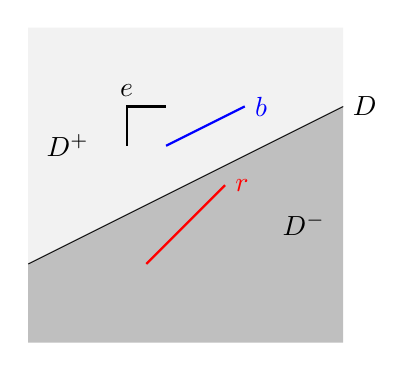
\begin{tikzpicture}
      \draw (-2, -1) -- (2, 1) node[right] {$D$};
      \fill [black, nearly transparent] %
      (-2, -1) -- (2, 1) -- (2, -2) -- (-2, -2) -- cycle;
      \draw (1.5, -0.5) node {$D^-$};
      \fill [black!20, nearly transparent] %
      (-2, -1) -- (2, 1) -- (2, 2) -- (-2, 2) -- cycle;
      \draw (-1.5, 0.5) node {$D^+$};
      \draw [thick](-0.75, 1) -- (-0.75, 0.5) -- (-0.75, 1)%
      node[above] {$e$} -- (-0.25, 1) ;
      \draw [blue, thick] (-0.25, 0.5) -- (0.75, 1) node[right] {$b$};
      \draw [red, thick] (-0.5, -1) -- (0.5, 0) node[right] {$r$};
    \end{tikzpicture}
\end{center}
\end{figure}

%%% Local Variables:
%%% mode: latex
%%% TeX-master: "../rapportGp1"
%%% End:


Si $e$ se trouve sur la droite $D$, alors aucun segment de $D$ n'est affiché;
tout segment sur la droite est réduit à un point vis-à-vis de $e$ et donc n'est
pas visible. L'ordre de traitement des demi-plans $D^+$ et $D^-$ n'importe
pas dans ce cas.

Se référer à l'algorithme \ref{algo:painter}.

\begin{algorithm}
  \caption{PaintersAlgorithm($T$, $e$)}
  \begin{algorithmic}[1] \label{algo:painter}
    \REQUIRE Un arbre BSP $T$ et un oeil $e$ (dont la position est $p=(x, y)$)
    \ENSURE -- (la scène représentée par $T$ est visualisée par $e$)
    \IF{$S\neq\varnothing$}
    \STATE $D\leftarrow$ la droite stockée en $T$
    \IF{$p\in D^+$}
    \STATE PaintersAlgorithm($T^-$, $e$)
    \STATE Visualiser les objets dans $S$
    \STATE PaintersAlgorithm($T^+$, $e$)
    \ELSIF{$p\in D^-$}
    \STATE PaintersAlgorithm($T^+$, $e$)
    \STATE Visualiser les objets dans $S$
    \STATE PaintersAlgorithm($T^-$, $e$)
    \ELSE
    \STATE PaintersAlgorithm($T^+$, $e$)
    \STATE PaintersAlgorithm($T^-$, $e$)
    \ENDIF
    \ENDIF
  \end{algorithmic}
\end{algorithm}

\begin{prop}[Complexité de l'algorithme du peintre dans le pire des cas]\label{compl:painter}
  Sous l'hypothèse que la visualisation des segments s'effectue
  en temps constant, l'algorithme du peintre est linéaire en le
  nombre de fragments de segments contenus dans $T$.
\end{prop}
\begin{proof}
  Procédons à une analyse du nombre de noeuds visités et du travail local
  par noeud.
  \begin{itemize}
  \item \textbf{Travail local par feuille}: par construction, une feuille
    ne contient aucun segment. La seule opération effectuée est le test
    $S\neq \varnothing$, qui est réalisé en temps constant $O(1)$.
  \item \textbf{Travail local par noeud interne}: si l'oeil est sur la droite
    stockée en le noeud, alors aucun travail n'est effectué. Donc dans le
    pire des cas, l'oeil ne se trouve sur aucune des droites de séparation.

    Chaque segment stocké dans l'ensemble $S$ est traité par l'oeil en
    temps constant. Dès lors, le travail local est en $O(\mathrm{Card}(S))$.
  \end{itemize}
  Tous les noeuds de l'arbre sont visités. Soient $n_I$ le nombre de noeuds
  internes de $T$, $n_F$ le nombre de feuilles de $T$, $V_I$ l'ensemble des
  noeuds internes de $T$ et $N$ le nombre
  de fragments stockés dans $T$.
  Pour $v\in V_I$, on note $S_v$ l'ensemble des segments stockés en ce noeud.

  Puisque $n_F \leq n_I + 1$, et que $n_I\leq N$,
  la complexité de l'algorithme est:
  $$ \sum_{v\in V_I}\left(\mathrm{Card}(S_v)\times O(1)\right) +
  n_I \times O(1) \leq O(N) + O(N) = O(N)$$
\end{proof}

Ce résultat permet l'observation suivante:
\begin{cor}\label{peintre:cor}
  L'efficacité de l'algorithme du peintre dépend directement
  du nombre de fragments générés par la construction de $T$.
\end{cor}
\subsection{Calcul des parties visibles}\label{not:oeil}
Cette section explique la procédure mise en \oe{}uvre pour déterminer
quelle proportion d'un segment est visible, étant donné un \oe{}il.
Après introduction des notations, des critères de visibilités sont
établis, suivis de l'élaboration d'une procédure pour calculer la
proportion du champ de vision occupée par un segment donné.

\subsubsection*{Notations et terminologie}
Tout au long de cette section, nous considérons un \oe{}il $e$, qui est la donnée à
la fois d'un point $(x, y)$ du plan représentant sa position et d'un angle $\phi$
qui représente la direction de vue de l'oeil. Autrement dit, l'orientation de
l'oeil est donnée par le vecteur $d=(\cos(\phi), \sin(\phi))$. Dans le modèle
adopté, l'oeil a une ouverture de $\pi/2$ radians. L'idée est de ramener
les segments visibles sur un arc de cercle et d'évaluer la proportion d'arc
à colorer. Une illustration de ce modèle est présentée à la figure \ref{oeil:ill}.

\begin{figure}[!h]
  \begin{center}
    \caption{Illustration d'un oeil}%
    \label{oeil:ill}
    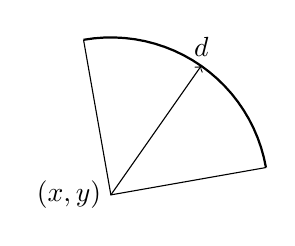
\begin{tikzpicture}
      \begin{scope}[rotate=10]
        \draw (2, 0) -- (0, 0) node[left] {$(x, y$)}-- (0, 2);
        \draw [->] (0, 0) -- (1.41421, 1.41421) node[above] {$d$};
        \draw [thick,domain=0:90] plot ({2*cos(\x)}, {2*sin(\x)});
      \end{scope}
    \end{tikzpicture}
\end{center}
\end{figure}
%%% Local Variables:
%%% mode: latex
%%% TeX-master: "../rapportGp1"
%%% End:


Sans perte de généralité, on peut supposer que $(x, y) = (0, 0)$;
si ce n'est pas le cas, tous les
calculs peuvent être effectués après une translation de $-(x, y)$ de tous
les objets considérés (notez que cette translation est une opération en $O(1)$).

La norme euclidienne d'un vecteur $v = (v_1, v_2)$ est notée
$\|v\|$ et vaut $\sqrt{v_1^2 + v_2^2}$. Au vu de la formule fondamentale liant le
sinus au cosinus, $\|d\| = 1$.

La notation $\langle \cdot,\cdot\rangle$ est employée pour le produit
scalaire usuel dans $\mathbb R^2$. Pour rappel,
pour tous $v=(v_1, v_2)$, $w=(w_1, w_2)\in\mathbb R^2$, on définit
$$\langle v, w\rangle = v_1 w_1 + v_2 w_2 = \|v\|\cdot\|w\|\cdot\cos(\theta)$$
où $\theta$ est l'angle entre les vecteurs $v$ et $w$.


\'Etant  donnés un vecteur $n = (a, b)$ et une droite $D\equiv ax+by=c$
(dont $n$ est un vecteur normal) il sera parfois dit
\og un objet est au-dessus de la droite $D$ relativement à la direction $n$\fg{}
plutôt que \og{}un objet est élément (ou est inclus) au demi-plan positif $D^+$\fg{}.
En effet, cela permet un vocabulaire plus imagé tout en restant cohérent
avec la réalité mathématique (un exemple est donné à la figure \ref{sep:ill}).

Une équation de droite de $D$ peut également être donnée via le produit scalaire;
si la droite $D$ passe par le point $p$, alors une équation est donnée par
$\langle w, n\rangle = \langle p, n\rangle$ où $w=(w_1, w_2)\in\mathbb R^2$ est
la variable de l'équation et $n$ désigne un vecteur normal à $D$.

Dans la suite, la droite de direction $d$ et passant par $(0, 0)$ est notée $D$.
\subsubsection*{Région de points visibles}
L'ensemble des points visibles est par définition l'ensemble
des vecteurs\footnote{On identifie un point du plan au vecteur
  joignant l'origine à ce point.} $v$ tel que l'angle non orienté formé
par $v$ et $d$ est inférieur à $\pi/4$.

Il s'agit également de la région délimitée par les demi-droites d'extrémité
$(0, 0)$ dont les directions et sens respectifs sont donnés par
$d_1 = (\cos(\phi + \pi/4), \sin(\phi + \pi/4))$ et
$d_2 = (\cos(\phi - \pi/4), \sin(\phi - \pi/4))$.

Notez que $d_1$ est un vecteur
normal de la demi-droite de direction $d_2$ et réciproquement.
Soient la droite $D_1$ (resp. $D_2$) de vecteur directeur $d_1$
(resp. $d_2$). Il est important de remarquer
que le demi-plan en dessous de $D_1$ (resp. $D_2$) relativement au vecteur
normal $d_2$ (resp. $d_1$) est un sous-ensemble convexe de points non visibles.
Une illustration est fournie à la figure \ref{vis:ill}.

\begin{figure}[!h]
  \begin{center}
    \caption{Illustration des différents vecteurs introduits}%
    \label{vis:ill}
    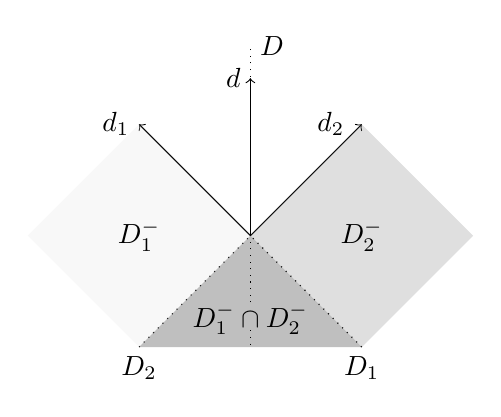
\begin{tikzpicture}
      \begin{scope}[rotate=45]
        \draw [<-] (2, 0) node[left] {$d_2$\phantom{i}} -- (0, 0);
        \draw [dotted] (-2, 0) node[below] {$D_2$} -- (0, 0);
        \draw [->] (0, 0)-- (0, 2) node[left] {$d_1$};
        \draw [dotted] (0, -2) node[below] {$D_1$} -- (0, 0);
        \draw [->] (0, 0) -- (1.41421, 1.41421) node[left] {$d$};
        \fill [black!50, nearly transparent](0, 0) -- (2, 0) -- (2, -2)%
        -- (0, -2) -- cycle;
        \fill [black!10, nearly transparent](0, 0) -- (-2, 0) -- (-2, 2)%
        -- (0, 2) -- cycle;
        \fill [black, nearly transparent] (0, 0) -- (0, -2) -- (-2, 0) -- cycle;
        \draw (-1, 1) node{$D_1^-$};
        \draw (1, -1) node{$D_2^-$};
        \draw (-0.75, -0.75) node {$D_1^-\cap D^-_2$};
        \draw [dotted] (-0.6, -0.6)  -- (1.7, 1.7) node[right] {$D$};
        \draw [dotted] (-0.85, -0.85)  -- (-1, -1);
      \end{scope}
    \end{tikzpicture}
\end{center}
\end{figure}
%%% Local Variables:
%%% mode: latex
%%% TeX-master: "../rapportGp1"
%%% End:

\subsubsection*{Critère de visibilité}
Soient $p_i=(u_i, v_i)\in\mathbb R^2$, $i = 1$, $2$ deux points du plan. Ici, nous nous
intéressons à la question \og\emph{existe-t-il une partie du segment $[p_1, p_2]$
  visible par $e$?}\fg.

Avant d'étudier la question pour un segment entier, il est intéressant de
se réduire au cas d'un point $p$ du plan, différent de l'origine:
$p$ est dans le cône de vision de $e$
si et seulement si l'angle (non orienté) entre la direction
$d$ de l'\oe{}il et le vecteur $p$
est inférieur
à $\pi/4$. Ceci découle simplement de la définition de $e$ et de son ouverture
de $\pi/2$ radians.

\begin{lem}\label{lem:angle}
  La complexité en temps du calcul d'un angle entre un vecteur $p\in\mathbb R^2$
  et $d$ est $O(1)$.
\end{lem}
\begin{proof}
  Soit $\theta$ l'angle non orienté entre $p$ et $d$.
  Dès lors, par définition du produit scalaire,
  $\cos(\theta) = \langle p, d\rangle/\|d\|$. L'emploi de $\arccos$
  fournit l'angle non orienté recherché.

  Signer l'angle revient à déterminer
  dans quel demi-plan par rapport à la droite $D$ se trouve $p$.
  Au vu du lemme \ref{lem:droite}, la détermination de l'équation de $D$
  peut être effectuée en temps constant et il en va de même pour l'évaluation
  de la fonction associée à la droite.

  \'Etant donné que seules des opérations mathématiques interviennent,
  la complexité de la détermination d'un angle entre $p$ et $d$ est $O(1)$.
\end{proof}

Dès qu'une des deux extrémités du segment $[p_1, p_2]$ appartient au
cône visible par l'\oe{}il, le segment est (partiellement)
visible. Il reste à étudier les configurations où ni $p_1$, ni $p_2$ ne sont
visibles, mais le segment est tout de même partiellement dans le champ de vision.

Deux configurations symétriques sont immédiatement à rejeter.
\begin{obs}\label{obs:side}
  Si $p_1$ et $p_2$ se trouvent dans le même demi-plan par rapport à $D$,
  et sont tous les deux hors de vue, alors le segment est complètement hors de vue.
\end{obs}
\begin{proof}
  Pour ne pas s'encombrer de lourdes notations, la preuve est effectuée
  géométriquement.

  Sous ces hypothèses, les extrémités sont comprises dans l'intersection
  de deux convexes du plan; le demi-plan relatif à $D$ et $D_i^-$ où la valeur
  de $i$ à choisir est dépendante du demi-plan relatif à $D$ considéré.
  Sur la figure \ref{vis:ill}, si les extrémités du segments étaient
  à gauche relativement à $D$, alors elles seraient dans $D_1^-$ et
  si elles étaient à droite, elles seraient dans $D_2^-$.

  Ces deux demi-plans étant convexes, dans le premier cas le
  segment serait contenu dans le demi-plan $D_1^-$ et dans le second
  cas, il serait contenu dans le demi-plan $D_2^-$.
\end{proof}

Il reste à traiter les configurations dans lesquelles $p_1$
et $p_2$ sont dans des demi-plans différents par rapport à $D$.

\begin{obs}\label{obs:couvr}
  Soit $D$ la droite de direction $d$ et passant par $(0, 0)$.
  Supposons que les extrémités $p_1$ et $p_2$ se trouvent
  de part et d'autre de $D$ et ne sont pas visibles.
  Alors le segment est partiellement visible
  si et seulement si la droite passant par $p_1$
  et $p_2$ est \og au-dessus\fg{} de $e$ relativement à $d$.

  De plus, la seule possibilité si le segment est partiellement
  visible est qu'il occupe tout le champ de vision.
\end{obs}

\begin{proof}
  Soit $n\perp d$ un vecteur normal à $d$. Soit $B$ la base $(d, n)$
  de $\mathbb R^2$. Affirmer qu'un point $p$ se trouve
  dans le demi-plan au-dessus de $e$ relativement à $d$ revient à dire
  que la composante $d$ de $p$ dans la base $B$ est strictement
  positive. Par passer au-dessus de $e$, on entend avoir comme coordonnées
  $(\lambda, 0)$ pour un $\lambda >0$ dans la base $B$, et dans le cas d'une
  droite, on entend avoir un point vérifiant cela.
  Les hypothèses assurent que le signe de la composante $n$ dans la base
  $(d, n)$ de $p_1$ et $p_2$ sont opposés.

  Supposons que le segment soit partiellement visible. Le théorème
  des valeurs intermédiaires assure qu'il existe un point $q$ du segment
  $[p_1, p_2]$ dont la composante $n$ dans $B$ est nulle. Si la
  composante $d$ de ce point était négative (\emph{ie}. par l'absurde,
  on suppose que le segment n'a aucun point au-dessus de l'oeil),
  alors il ne serait pas visible par l'observation \ref{obs:side} 
  car aucune de ses moitiés $[p_1, q]$ et$[q, p_2]$ ne seraient visibles.

  Si la droite passe au-dessus de $e$, il est immédiat que le segment
  est partiellement visible.

  Il reste à montrer que si une de ces assertions est vérifiée, alors
  tout la vision est occupée par le segment. Or, le segment
  $[p_1, p_2]$ intersecte les droites $D_1$ et $D_2$ dans le demi-plan
  au-dessus de $e$ relativement à $d$ car le segment contient un point
  au-dessus de $e$. Ceci assure que la vue est recouverte.
\end{proof}
\begin{lem}\label{lem:couvr}
  La vérification de l'observation \ref{obs:couvr} peut être effectuée en
  temps constant.
\end{lem}
\begin{proof}
  Quitte à échanger $p_1$ et $p_2$, on peut supposer $p_1$ à gauche
  (en imaginant que $d$ indique le haut) de la droite $D$.
  Soit $n$ le vecteur joignant $p_2$ à $p_1$ auquel est appliqué
  une rotation de $\pi/2$ vers la droite, c'est-à-dire la fonction
  $$ \rho_{-\pi/2}:\mathbb R^2\to\mathbb R^2: (u, v)\mapsto (v, -u),$$
  alors l'équation de droite $\langle w, n\rangle = \langle p_1, n\rangle$
  est une équation de la droite passant par $p_1$ et $p_2$.
  Si $\langle p_1, n\rangle$ est positif, alors la droite passe au-dessus
  de l'origine.

  \'Etant donné que seules des opérations arithmétiques et des comparaisons
  sont effectuées, ce calcul s'effectue en temps constant.
\end{proof}

\subsubsection*{Calcul de proportion visible}
Afin d'afficher la portion visible du segment,
il suffit de déterminer quelle proportion d'arc  porte la couleur du segment.
Pour ramener les segments sur le cercle trigonométrique, il suffit
de ramener les extrémités sur le cercle en les normalisant (c'est-à-dire en
les divisant par leur norme) et
de colorer l'arc de longueur moindre entre les points.
L'idée sous-jacente est qu'aucun angle au centre d'un cercle ne
peut excéder $\pi$ radians.
\begin{figure}[!h]
  \begin{center}
    \caption{Configurations possibles sous l'hypothèse qu'un point est visible}%
    \label{config:ill}
    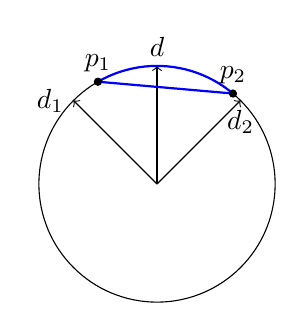
\begin{tikzpicture}[scale=1.5]
      \draw [thin] (0, 0) circle (1cm);
      \draw [->](0, 0) -- (90:1) node[above] {$d$};
      \draw [->] (0, 0) -- (45:1) node[below] {$d_2$};
      \draw [->] (0, 0) -- (135:1) node[left] {$d_1$};
      \draw [blue, thick, domain=50:120] plot ({cos(\x)}, {sin(\x)});
      \draw [thick, blue] (120:1) -- (50:1);
      \draw [thin, fill=black] (120:1) circle (0.03cm) node[above] {$p_1$};
      \draw [thin, fill=black] (50:1) circle (0.03cm) node[above] {$p_2$};
    \end{tikzpicture}
    % \begin{tikzpicture}[scale=1.5]
    %   \draw [thin] (0, 0) circle (1cm);
    %   \draw [->](0, 0) -- (90:1) node[above] {$d$};
    %   \draw [->] (0, 0) -- (45:1) node[above] {$d_2$};
    %   \draw [->] (0, 0) -- (135:1) node[above] {$d_1$};
    %   \draw [blue, thick, domain=-15:70] plot ({cos(\x)}, {sin(\x)});
    %   \draw [thick, blue] (-15:1) -- (70:1);
    % \end{tikzpicture}
    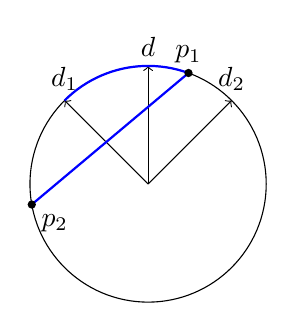
\begin{tikzpicture}[scale=1.5]
      \draw [thin] (0, 0) circle (1cm);
      \draw [->](0, 0) -- (90:1) node[above] {$d$};
      \draw [->] (0, 0) -- (45:1) node[above] {$d_2$};
      \draw [->] (0, 0) -- (135:1) node[above] {$d_1$};
      \draw [blue, thick, domain=70:135] plot ({cos(\x)}, {sin(\x)});
      \draw [thick, blue] (190:1) -- (70:1);
      \draw [thin, fill=black] (190:1) circle (0.03cm) node[below right]{$p_2$};
      \draw [thin, fill=black] (70:1) circle (0.03cm) node[above] {$p_1$};
    \end{tikzpicture}
    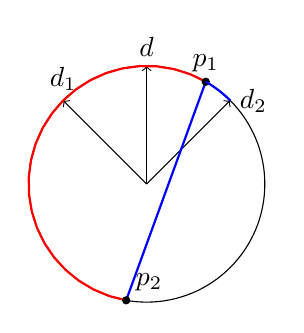
\begin{tikzpicture}[scale=1.5]
      \draw [thin] (0, 0) circle (1cm);
      \draw [->](0, 0) -- (90:1) node[above] {$d$};
      \draw [->] (0, 0) -- (45:1) node[right] {$d_2$};
      \draw [->] (0, 0) -- (135:1) node[above] {$d_1$};
      \draw [red, thick, domain=60:260] plot ({cos(\x)}, {sin(\x)});
      \draw [thick, blue] (260:1) -- (60:1);
      \draw [thin, fill=black] (260:1) circle (0.03cm) node[above right]{$p_2$};
      \draw [thin, fill=black] (60:1) circle (0.03cm) node[above]{$p_1$};
      \draw [blue, thick, domain=45:60] plot ({cos(\x)}, {sin(\x)});
    \end{tikzpicture}
\end{center}
\end{figure}
%%% Local Variables:
%%% mode: latex
%%% TeX-master: "../rapportGp1"
%%% End:


Le segment représentant la vue de l'\oe{}il est identifié à l'intervalle
$[0, 1]$. Après détermination des angles définissant l'arc de cercle
à colorer, la bijection décroissante suivante est utilisée pour
se ramener à l'intervalle $[0, 1]$:
$$f:\left[-\frac{\pi}{4}, \frac{\pi}{4}\right]\to [0, 1]: \theta \mapsto 1 - \frac{2}{\pi}\left(\theta + \frac{\pi}{4}\right).$$

La décroissance est imposée car l'accroissement des angles mène
à une rotation vers la gauche alors que croître dans l'intervalle
revient à avancer vers la droite.

Soient $\theta_1$ et $\theta_2$ les angles \emph{signés}
entre $d$ et $p_1$ et $p_2$
respectivement. Supposons que $\theta_1$ est dans l'intervalle $[-\pi/4, \pi/4]$
(autrement dit $p_1$ est visible). Il n'est pas nécessaire de considérer
les autres cas au vu de la section précédente. Les cas à distinguer selon
$\theta_2$ sont les suivants:

\begin{itemize}
  \item Si $\theta_2\in[-\pi/4, \pi/4]$, la partie à colorer de $[0, 1]$ est
    l'intervalle (non orienté) $[f(\theta_1), f(\theta_2)]$
    (se référer à la première illustration de la figure \ref{config:ill}).
  \item Sinon, si $|\theta_2|>\pi/4$ et $|\theta_1-\theta_2|\leq \pi$,
    on colore l'intervalle $[f(\theta_1), 1]$ si $\theta_2<-\pi/4$ et
    $[0, f(\theta_1)]$ si $\theta_2>\pi/4$
    (voir la deuxième illustration de la figure \ref{config:ill}).
  \item Sinon, si $|\theta_2|>\pi/4$ et $|\theta_1-\theta_2|> \pi$,
    on colore l'intervalle $[0, f(\theta_1)]$ si $\theta_2<-\pi/4$ et
    $[f(\theta_1), 1]$ si $\theta_2>\pi/4$. La dernière illustration
    de la figure \ref{config:ill} exemplifie cette situation. L'arc
    de longueur $|\theta_1-\theta_2|$ est dessiné en rouge
    pour le mettre en évidence.
\end{itemize}

\subsubsection*{Algorithmes}

Afin d'effectuer les calculs de complexités pour la procédure
de visualisation, les algorithmes associés sont présentés
dans cette section.

\begin{algorithm}
  \caption{estVisible($s=[p_1, p_2]$, $e$)}\label{algo:estvis}
  \begin{algorithmic}[1]
    \REQUIRE Un oeil $e$ positionné en $(0, 0)$ d'angle $\phi$ et un segment $s$
    donné par ses extrémités $p_1$, $p_2$.
    \ENSURE un signal indiquant si le segment a une extrémité visible,
    s'il obstrue complètement la vue ou s'il n'est pas visible.
    \STATE $d\leftarrow (\cos(\phi), \sin(\phi))$
    \STATE $\theta_1\leftarrow$ l'angle entre $d$ et $p_1$ \label{r1:estvis}
    \STATE $\theta_2\leftarrow$ l'angle entre $d$ et $p_2$ \label{r2:estvis}
    \IF{$\theta_1\in[-\pi/4, \pi/4]\lor \theta_2\in[-\pi/4, \pi/4]$}
    \RETURN \og{}une extrémité est visible\fg{}
    \ELSIF{$\theta_1$ et $\theta_2$ ont le même signe}
    \RETURN \og le segment n'est pas visible \fg \\
    \COMMENT{les extrémités sont dans le même demi-plan par rapport à $D$}
    \ELSIF{la droite passant par $p_1$ et $p_2$ est au-dessus de $(0, 0)$ relativement à $d$} \label{r3:estvis}
    \RETURN \og le segment couvre la vue\fg
    \ELSE
    \RETURN \og le segment n'est pas visible \fg
    \ENDIF
  \end{algorithmic}
\end{algorithm}

\begin{prop}
  La complexité de l'algorithme \ref{algo:estvis} est $O(1)$.
\end{prop}
\begin{proof}
  Les lemmes \ref{lem:angle} et \ref{lem:couvr} assurent que
  les instructions \ref{r1:estvis}, \ref{r2:estvis} et \ref{r3:estvis} sont en temps
  constant. Les autres instructions sont toutes en temps constant, car il s'agit
  de comparaisons de nombres.
\end{proof}

\begin{algorithm}
  \caption{proportionVisible($e$, $s$)}
  \begin{algorithmic}[1] \label{algo:propvis}
    \REQUIRE Un oeil $e$ positionné en $(0, 0)$ d'angle $\phi$ et un segment $s$
    donné par ses extrémités $p_1$, $p_2$ dont une des extrémités est visible.
    \ENSURE un couple de réels entre $0$ et $1$  indiquant le sous-intervalle
    non-orienté de vue occupé par $s$.
    \STATE $d\leftarrow (\cos(\phi), \sin(\phi))$
    \STATE $\theta_1\leftarrow$ l'angle entre $d$ et $p_1$ \label{r1:propvis}
    \STATE $\theta_2\leftarrow$ l'angle entre $d$ et $p_2$ \label{r2:propvis}
    \STATE $f\leftarrow$ la fonction $
    [-\pi/4, \pi/4]\to [0, 1]: x\mapsto 1 - (x+\pi/4) \times 2/\pi$
    \IF{$\theta_1\in[-\pi/4, \pi/4]\land \theta_2\in[-\pi/4, \pi/4]$}
    \RETURN $(f(\theta_1), f(\theta_2))$
    \ELSE
    \IF{$\theta_1\notin[-\pi/4, \pi/4]$}
    \STATE échanger $\theta_1$ et $\theta_2$
    \COMMENT{ceci assure que $\theta_1\in[-\pi/4, \pi/4]$ et
      $\theta_2\notin[-\pi/4, \pi/4]$}
    \ENDIF
    \IF{$|\theta_1-\theta_2|\leq\pi$}
    \IF{$\theta_2>\pi/4$}
    \RETURN $(0, f(\theta_1))$
    \ELSE
    \RETURN $(f(\theta_1), 1)$
    \ENDIF
    \ELSIF{$|\theta_1-\theta_2|>\pi$}
    \IF{$\theta_2>\pi/4$}
    \RETURN $(f(\theta_1), 1)$
    \ELSE
    \RETURN $(0, f(\theta_1))$
    \ENDIF
    \ENDIF
    \ENDIF
  \end{algorithmic}
\end{algorithm}

\begin{prop}
  La complexité de l'algorithme \ref{algo:propvis} est $O(1)$.
\end{prop}
\begin{proof}
  Le lemme \ref{lem:angle} assure que les instructions \ref{r1:propvis} et
  \ref{r2:propvis} sont en temps constant. Le calcul de la fonction $f$
  est également réalisée en temps constant. Les différentes instructions
  conditionnelles étant toutes également en $O(1)$, la complexité de
  l'algorithme est bien $O(1)$.
\end{proof}



%%%Local Variables:
%%% mode: latex
%%% TeX-master: "../rapportGp1"
%%% End:
